\chapter{Valutazione dei risultati e metriche di qualità} \label{chap:evaluation}

Questo capitolo presenta le metriche comunemente utilizzate in astrofotografia, nonché quelle impiegate in questo progetto per valutare la qualità delle immagini ottenute attraverso il processo di elaborazione descritto nei capitoli precedenti.

La selezione delle metriche è fondamentale per stabilire criteri oggettivi di valutazione e per confrontare i risultati ottenuti con diverse configurazioni di parametri. Verranno discusse sia metriche con riferimento, che richiedono un'immagine ideale per il confronto, sia metriche senza riferimento, che valutano autonomamente la qualità dell'immagine

Successivamente, verranno presentati i risultati ottenuti e analizzati i miglioramenti introdotti dalle varie tecniche di elaborazione delle immagini.


\section{Metriche di valutazione con riferimento} \label{sec:r_metrics}

Le metriche con riferimento confrontano l'immagine elaborata con un'immagine ideale, fornendo una misura della similarità o della qualità relativa tra le due. Nel contesto di questo progetto, l'utilizzo di metriche con riferimento ha presentato alcune sfide, principalmente a causa dell'assenza di un'immagine di riferimento adeguata, come discusso nella \cref{sec:challenges}.

\subsection{SSIM} \label{subsec:ssim}

\textbf{SSIM} (Structural Similarity Index Measure) è una metrica che misura la similarità strutturale tra due immagini. In astrofotografia, dopo aver applicato tecniche di denoising, la metrica SSIM viene utilizzata per valutare quanto efficacemente il rumore è stato ridotto mantenendo intatte le strutture originali dell'immagine, come stelle, galassie e nebulose. SSIM può essere impiegata anche per perfezionare la tecnica dello stacking, aiutando a determinare quali combinazioni di immagini offrono la migliore preservazione delle strutture dettagliate rispetto all'immagine di riferimento.

La formula generale per il calcolo dell'SSIM tra due immagini $x$ e $y$ è:

$$
\text{SSIM}(x, y) = \frac{(2\mu_x\mu_y + C_1)(2\sigma_{xy} + C_2)}{(\mu_x^2 + \mu_y^2 + C_1)(\sigma_x^2 + \sigma_y^2 + C_2)}
$$

dove $\mu_x$ e $\mu_y$ sono le medie delle immagini $x$ e $y$, $\sigma_x^2$ e $\sigma_y^2$ sono le varianze, $\sigma_{xy}$ è la covarianza tra $x$ e $y$ e, infine, $C_1$ e $C_2$ sono due costanti che stabilizzano la divisione in caso di valori molto bassi di $\mu_x^2 + \mu_y^2$ e $\sigma_x^2 + \sigma_y^2$. Il valore dell'SSIM è compreso tra $-1$ e $1$, dove $1$ indica una similarità perfetta tra le due immagini, e $-1$ indica una dissimilarità totale.

SSIM tiene conto della percezione umana, valutando la luminanza, il contrasto e la struttura delle immagini. Tuttavia, è sensibile a piccoli spostamenti e rotazioni tra le immagini e non è in grado di valutare la qualità di immagini con diverse dimensioni o scale.

Nel progetto, a causa dell'assenza di un'immagine di riferimento adeguata (come discusso nella \cref{sec:challenges}), l'utilizzo dell'SSIM non è stato possibile.

\subsection{SNR} \label{subsec:snr}

Il \textbf{Rapporto Segnale-Rumore} (SNR: Signal-to-Noise Ratio) è una metrica fondamentale nell'ambito dell'astrofotografia, utilizzata per quantificare la qualità delle immagini astronomiche. Esso misura la relazione tra il segnale utile (le informazioni desiderate, come stelle, galassie o, in questo caso, la Luna e i suoi dettagli) e il rumore di fondo presente nell'immagine. Un alto valore di SNR indica che il segnale è dominante rispetto al rumore, risultando in immagini più nitide e dettagliate. 

Generalmente l'SNR si calcola a partire dalla normalizzazione dell'errore quadratico medio o di altre metriche di errore relative, come segue:

$$
SNR = 10 \cdot \log_{10} (\xi)
$$

$\xi$ è l'errore relativo calcolato scondo formule come:

\begin{enumerate}
    \item Normalized Least Squares Error (NLSE):
    $$
    \xi_{NLSE} = \dfrac{\sum_{j = 1}^J \sum_{k=1}^K |F(j, k) - \hat F(j, k)|^2}
    {\sum_{j = 1}^J \sum_{k=1}^K |F(j, k)|^2}
    $$

    \item Peak Least Squares Error (PLSE):
    $$
    \xi_{PLSE} = \dfrac{\sum_{j = 1}^J \sum_{k=1}^K |F(j, k) - \hat F(j, k)|^2}
    {[\text{MAX}\{F(j, k)\}]^2}
    $$
\end{enumerate}

dove $F(j, k)$ è il valore del pixel originale, $\hat F(j, k)$ è il valore del pixel elaborato, $J$ e $K$ sono le dimensioni dell'immagine e $\text{MAX}\{F(j, k)\}$ è il valore massimo del pixel nell'immagine originale.

Una formula semplificata e comunemente utilizzata per calcolare l'SNR è:

$$
SNR = 10\cdot \log_{10} \left(\dfrac{\mu_s^2}{\sigma_n^2}\right)
$$

dove $\mu_s$ è la media del segnale e $\sigma_n$ è la deviazione standard del rumore.

L'SNR è una metrica semplice e intuitiva, ma non tiene conto delle caratteristiche percettive del sistema visivo umano. Inoltre, come SSIM, è sensibile a piccoli spostamenti e rotazioni tra le immagini e non è in grado di valutare la qualità di immagini con diverse dimensioni o scale, richiedendo dunque un perfetto allineamento tra le immagini di riferimento e quelle elaborate.

Algoritmi di denoising avanzati, inclusi quelli basati su reti neurali, vengono valutati utilizzando l'SNR per garantire che il segnale sia preservato efficacemente mentre il rumore viene minimizzato. Tuttavia, anche l'SNR non è stato utilizzato in questo progetto a causa dell'assenza di un'immagine di riferimento adeguata.

\section{Metriche di valutazione senza riferimento} \label{sec:nr_metrics}

La mancanza di un'immagine di riferimento ideale ha reso necessario l'utilizzo di metriche di valutazione senza riferimento per valutare la qualità delle immagini elaborate.

Le metriche senza riferimento valutano la qualità dell'immagine in maniera autonoma, senza bisogno di confrontarla con un'immagine ideale,analizzando dunque l'immagine stessa per stimare la sua qualità basandosi su modelli statistici o percettivi.

\subsection{NIQE} \label{subsec:niqe}

\textbf{NIQE} (Naturalness Image Quality Evaluator) è una metrica di qualità delle immagini senza riferimento, sviluppata per valutare autonomamente la qualità delle immagini digitali, senza necessità di un'immagine di riferimento. NIQE è basata su un modello di percezione visiva umana, che valuta la qualità dell'immagine basandosi su caratteristiche statistiche e percettive, come la nitidezza, il contrasto, la luminosità e la presenza di artefatti \cite{niqe}.

NIQE calcola la distanza tra le statistiche dell'immagine e quelle di un campione di immagini di riferimento, fornendo un punteggio di qualità (generalmente tra 0 e 100) che indica quanto l'immagine si discosti dalla media delle immagini di riferimento. Punteggi più bassi indicano una qualità migliore.

Nel progetto, NIQE è stata testata come possibile metrica di valutazione, ma ha mostrato limitazioni nel catturare miglioramenti specifici apportati dalle tecniche di elaborazione applicate alle immagini lunari. Ciò è probabilmente dovuto alla natura specifica delle immagini lunari, che possono differire significativamente dalle immagini di riferimento utilizzate per addestrare il modello.

\subsection{BRISQUE} \label{subsec:brisque}

\textbf{BRISQUE} (Blind Referenceless Image Spatial Quality Evaluator) è una metrica di qualità delle immagini senza riferimento che valuta le distorsioni naturali basandosi su modelli statistici delle scene naturali \cite{brisque}. A differenza di NIQE, BRISQUE utilizza un approccio di apprendimento supervisionato, addestrato su un ampio dataset di immagini con varie distorsioni.

BRISQUE estrae caratteristiche statistiche dall'immagine, come la distribuzione dei coefficienti MSCN (Mean Subtracted Contrast Normalized), per catturare le deviazioni dalla naturalità statistica tipicamente presenti nelle immagini di alta qualità. Il modello produce un punteggio di qualità in una scala da 0 a 100, dove punteggi più bassi indicano una qualità migliore.

Nel contesto del progetto, BRISQUE ha dimostrato una maggiore sensibilità rispetto a NIQE nel rilevare miglioramenti nella qualità dell'immagine, ma ha presentato alcune limitazioni nell'analisi di immagini astronomiche, che differiscono significativamente dalle scene naturali su cui il modello è stato addestrato.

\subsection{LIQE} \label{subsec:liqe}

\textbf{LIQE} (Learning-based Image Quality Evaluator) è una metrica di qualità delle immagini senza riferimento basata su tecniche di \textit{deep learning} avanzate \cite{liqe}. LIQE si distingue per la sua capacità di combinare efficacemente informazioni statistiche a livello sia globale che locale, permettendo una valutazione più accurata delle distorsioni presenti nelle immagini.

Il modello assegna un punteggio in una scala da 1 a 5, dove 1 indica una qualità molto bassa e 5 una qualità molto alta. Questa scala è adottata nell'implementazione della libreria \texttt{PyIQA} utilizzata nel progetto; altre implementazioni possono utilizzare scale diverse (generalmente 0-100).

La caratteristica distintiva di LIQE rispetto a NIQE e BRISQUE è la sua architettura basata su reti neurali convoluzionali profonde, addestrate su un vasto dataset di immagini con varie distorsioni. Questo approccio rende LIQE particolarmente robusto e versatile nella valutazione di diverse tipologie di immagini, incluse quelle con caratteristiche non convenzionali come le immagini astronomiche.

Rispetto a NIQE e BRISQUE, LIQE è stato progettato per essere più robusto e generale e può essere utilizzato per valutare una vasta gamma di immagini. LIQE è stato addestrato su un dataset di immagini distorte e utilizza una rete neurale convoluzionale per valutare autonomamente la qualità delle immagini.

\subsection{Considerazioni sulle metriche} \label{subsec:why_liqe}

Nel progetto, sono state implementate e testate diverse metriche di valutazione senza riferimento, tra cui NIQE, BRISQUE e LIQE, utilizzando la libreria \texttt{PyIQA}, che fornisce implementazioni pronte all'uso di diverse metriche di qualità delle immagini.

Dopo aver valutato i risultati ottenuti, è emerso che \textbf{LIQE risulta la metrica più adatta} per valutare la qualità delle immagini lunari elaborate. La scelta di LIQE come metrica principale per la valutazione dei risultati è stata motivata da diversi fattori. Innanzitutto, a causa dell'assenza di un'immagine di riferimento ideale, le metriche con riferimento non erano applicabili nel contesto del progetto. Tra le metriche senza riferimento, LIQE ha dimostrato di essere più sensibile ai miglioramenti apportati dalle tecniche di elaborazione implementate.

Durante lo sviluppo, è emerso che metriche come NIQE e BRISQUE non sempre riflettevano accuratamente la percezione umana della qualità delle immagini. Ad esempio, in alcuni casi, un'immagine che visivamente appariva migliorata presentava un punteggio peggiore secondo queste metriche. LIQE, invece, ha mostrato una maggiore correlazione con la qualità percepita.

È importante notare che LIQE non è progettato per valutare immagini astronomiche. Il modello (che assegna vlori tra 1 e 5), assegna valori che si aggirano intorno a 2, indicando una qualità molto bassa. Probabilmente ciò è dovuto al fatto che il modello è stato addestrato su un dataset di immagini a colori, mentre la Luna è pressocché monocromatica. Tuttavia, nonostante queste limitazioni, si può notare che a miglioramenti visivi delle immagini corrispondevano incrementi nei punteggi LIQE.

\section{Analisi e miglioramenti ottenuti} \label{sec:analysis}

In questa sezione vengono analizzati i risultati ottenuti attraverso l'applicazione delle diverse tecniche di elaborazione descritte nei capitoli precedenti. L'obiettivo è valutare l'efficacia di ciascuna fase del processo nel migliorare la qualità delle immagini lunari, utilizzando le metriche di valutazione senza riferimento discusse nel \cref{chap:evaluation}. Verranno presentati grafici, tabelle e immagini illustrative per supportare l'analisi e facilitare il confronto tra i vari metodi.

\subsection{Effetti della calibrazione} \label{subsec:analysis_cal}

La calibrazione delle immagini è un passaggio fondamentale nell'astrofotografia per rimuovere artefatti strumentali e migliorare il rapporto segnale-rumore. In questa sezione si analizza l'impatto della calibrazione sulle immagini lunari acquisite, confrontando le metriche di qualità prima e dopo l'applicazione della calibrazione.

% [Inserire qui i grafici e le tabelle che mostrano i punteggi di NIQE, BRISQUE e LIQE per le immagini non calibrate e calibrate]

Dai dati raccolti, si osserva che la calibrazione non ha comportato un miglioramento significativo nelle metriche di qualità, suggerendo che le immagini originali erano già ben bilanciate e prive di distorsioni significative. 
%! ---------------- da finire -----------------

\subsection{Impatto del denoising} \label{subsec:analysis_den}

Il denoising è essenziale per attenuare il rumore presente nelle immagini senza degradare i dettagli importanti. Sono stati testati diversi metodi di denoising, tra cui DnCNN, filtro gaussiano, filtro bilaterale e filtro mediano. In questa sezione vengono confrontati i risultati ottenuti con ciascun metodo.

\begin{figure}[H]
    \centering
    \begin{subfigure}[t]{0.24\textwidth}
        \centering
        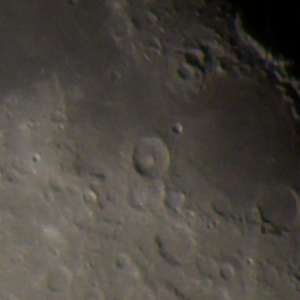
\includegraphics[width=\linewidth]{../assets/den_median_zoom.png}
        \caption{Filtro mediano}
        \label{fig:mediano}
    \end{subfigure}
    \hfill
    \begin{subfigure}[t]{0.24\textwidth}
        \centering
        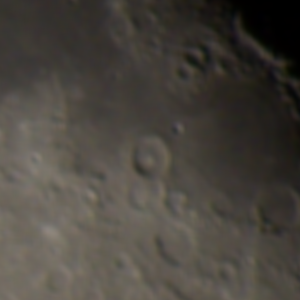
\includegraphics[width=\linewidth]{../assets/den_gaussian_zoom.png}
        \caption{Filtro gaussiano}
        \label{fig:gaussiano}
    \end{subfigure}
    \hfill
    \begin{subfigure}[t]{0.24\textwidth}
        \centering
        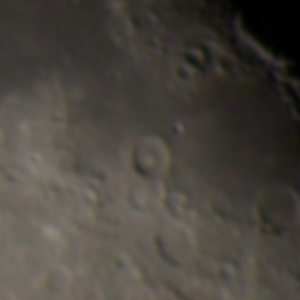
\includegraphics[width=\linewidth]{../assets/den_bilateral_zoom.png}
        \caption{Filtro bilaterale}
        \label{fig:bilaterale}
    \end{subfigure}
    \hfill
    \begin{subfigure}[t]{0.24\textwidth}
        \centering
        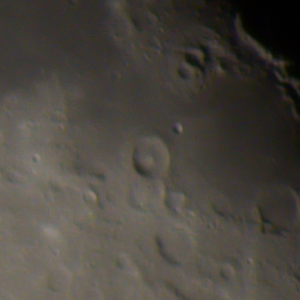
\includegraphics[width=\linewidth]{../assets/den_dncnn_zoom.png}
        \caption{DnCNN}
        \label{fig:dncnn}
    \end{subfigure}
    \caption{Confronto tra diversi filtri di riduzione del rumore.}
    \label{fig:confronto-filtri}
\end{figure}

\begin{figure}[H]
    \centering
    \begin{subfigure}[t]{0.45\textwidth}
        \centering
        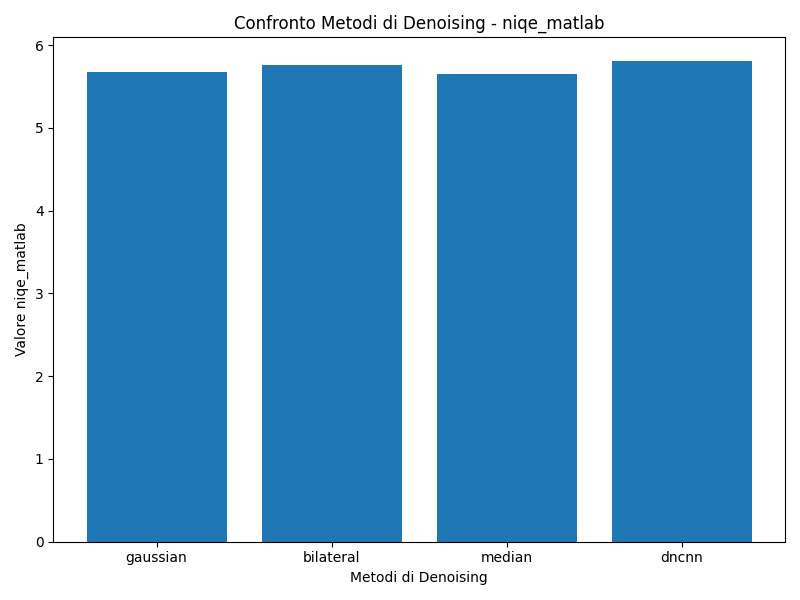
\includegraphics[width=\linewidth]{../assets/denoising_comparison_niqe_matlab.png}
        \caption{NIQE}
        \label{fig:den_niqe}
    \end{subfigure}
    \hfill
    \begin{subfigure}[t]{0.45\textwidth}
        \centering
        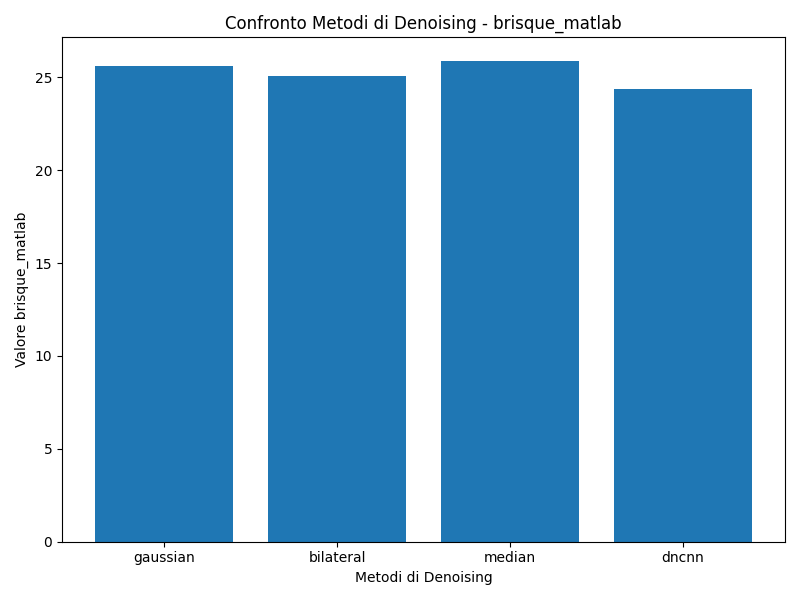
\includegraphics[width=\linewidth]{../assets/denoising_comparison_brisque_matlab.png}
        \caption{BRISQUE}
        \label{fig:den_brisque}
    \end{subfigure}
    \hfill
    \begin{subfigure}[t]{0.45\textwidth}
        \centering
        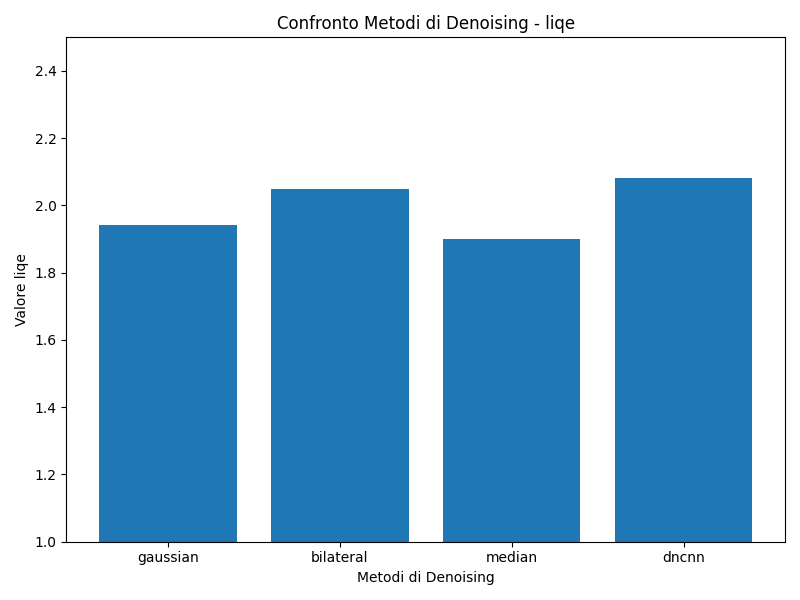
\includegraphics[width=\linewidth]{../assets/denoising_comparison_liqe.png}
        \caption{LIQE}
        \label{fig:den_liqe}
    \end{subfigure}
\end{figure}

L'analisi dei punteggi delle metriche e l'osservazione visiva delle immagini suggeriscono che il metodo DnCNN ha prodotto i migliori risultati in termini di riduzione del rumore mantenendo i dettagli. Tuttavia, alcuni metodi tradizionali come il filtro bilaterale hanno mostrato performance comparabili in determinate situazioni.

\subsection{Benefici dello stacking} \label{subsec:analysis_stack}

Lo stacking delle immagini consente di migliorare il rapporto segnale-rumore combinando più scatti dello stesso soggetto. Sono stati applicati diversi metodi di stacking: media pesata, mediana e sigma clipping. Inoltre, è stato analizzato l'effetto dell'aumento del numero di immagini utilizzate nello stacking.

% [Inserire grafici che mostrano come le metriche variano al variare del numero di immagini nello stacking]

% [Inserire tabelle o grafici che confrontano i metodi di stacking utilizzati]

I risultati evidenziano che l'incremento del numero di immagini nello stacking porta a un miglioramento nelle metriche di qualità, confermando l'efficacia di questa tecnica. Tra i metodi di stacking, la media pesata basata sulla nitidezza ha prodotto le immagini con la qualità complessiva migliore secondo le metriche utilizzate.

\subsection{Miglioramenti con sharpening e contrasto} \label{subsec:analysis_post}

Le tecniche di post-processing, come l'aumento della nitidezza tramite Unsharp Mask e il miglioramento del contrasto con CLAHE, sono state applicate alle immagini ottenute dopo lo stacking. In questa sezione si valutano gli effetti di queste tecniche sulla qualità finale delle immagini.

% [Inserire immagini che mostrano le differenze prima e dopo l'applicazione delle tecniche di post-processing]

% [Inserire punteggi delle metriche per le immagini pre e post-processing]

Dall'analisi emerge che l'applicazione dell'Unsharp Mask ha permesso di enfatizzare i dettagli superficiali della Luna, migliorando la nitidezza percepita. Il miglioramento del contrasto con CLAHE ha reso più visibili le variazioni tonali, contribuendo a una maggiore profondità dell'immagine. Le metriche di qualità riflettono questi miglioramenti, con punteggi più elevati nelle immagini post-processate.

\subsection{Analisi complessiva e discussione finale}

Combinando i risultati delle diverse fasi di elaborazione, si può valutare l'efficacia complessiva del processo sviluppato. Le immagini finali ottenute presentano un significativo miglioramento rispetto agli scatti originali, sia in termini di qualità percepita che secondo le metriche utilizzate.

% [Inserire qui una tabella riepilogativa con i punteggi delle metriche per le diverse fasi del processo]

È importante notare che le metriche utilizzate, pur essendo senza riferimento, hanno mostrato una buona correlazione con la qualità percepita delle immagini. Tuttavia, alcune limitazioni sono emerse, in particolare nella capacità delle metriche di catturare miglioramenti specifici legati alle caratteristiche uniche delle immagini lunari.

Le tecniche di elaborazione implementate si sono dimostrate efficaci nel contesto del progetto. La combinazione di calibrazione, denoising avanzato, stacking ottimizzato e post-processing ha permesso di ottenere immagini di alta qualità, evidenziando dettagli altrimenti non visibili.

% [Inserire considerazioni personali sull'efficacia delle tecniche, eventuali limitazioni riscontrate e possibili sviluppi futuri]

\cleardoublepage